\section{Software Design}
\subsection{Control and Monitoring system} 
\label{sec:monitoring}

For the first version of control and monitoring GUI, we will using QT framework 
with Python. Main features of the system is to monitor sensors data receive from MAVEN-01, velocity 
battery level and many other features. This system will information intuitively about the condition
of environments surround the rover which is the main target of MAVEN-01.

\vspace{1.5 em }
\href{https://www.qt.io/development/qt-framework}{QT framework} is flexible framework for making desktop application, compatible with both Python and C++,
more specific, MMS was using Pyside6, a library that allow users use QT APIS through Python. 

 \begin{figure}[H]
    \centering
    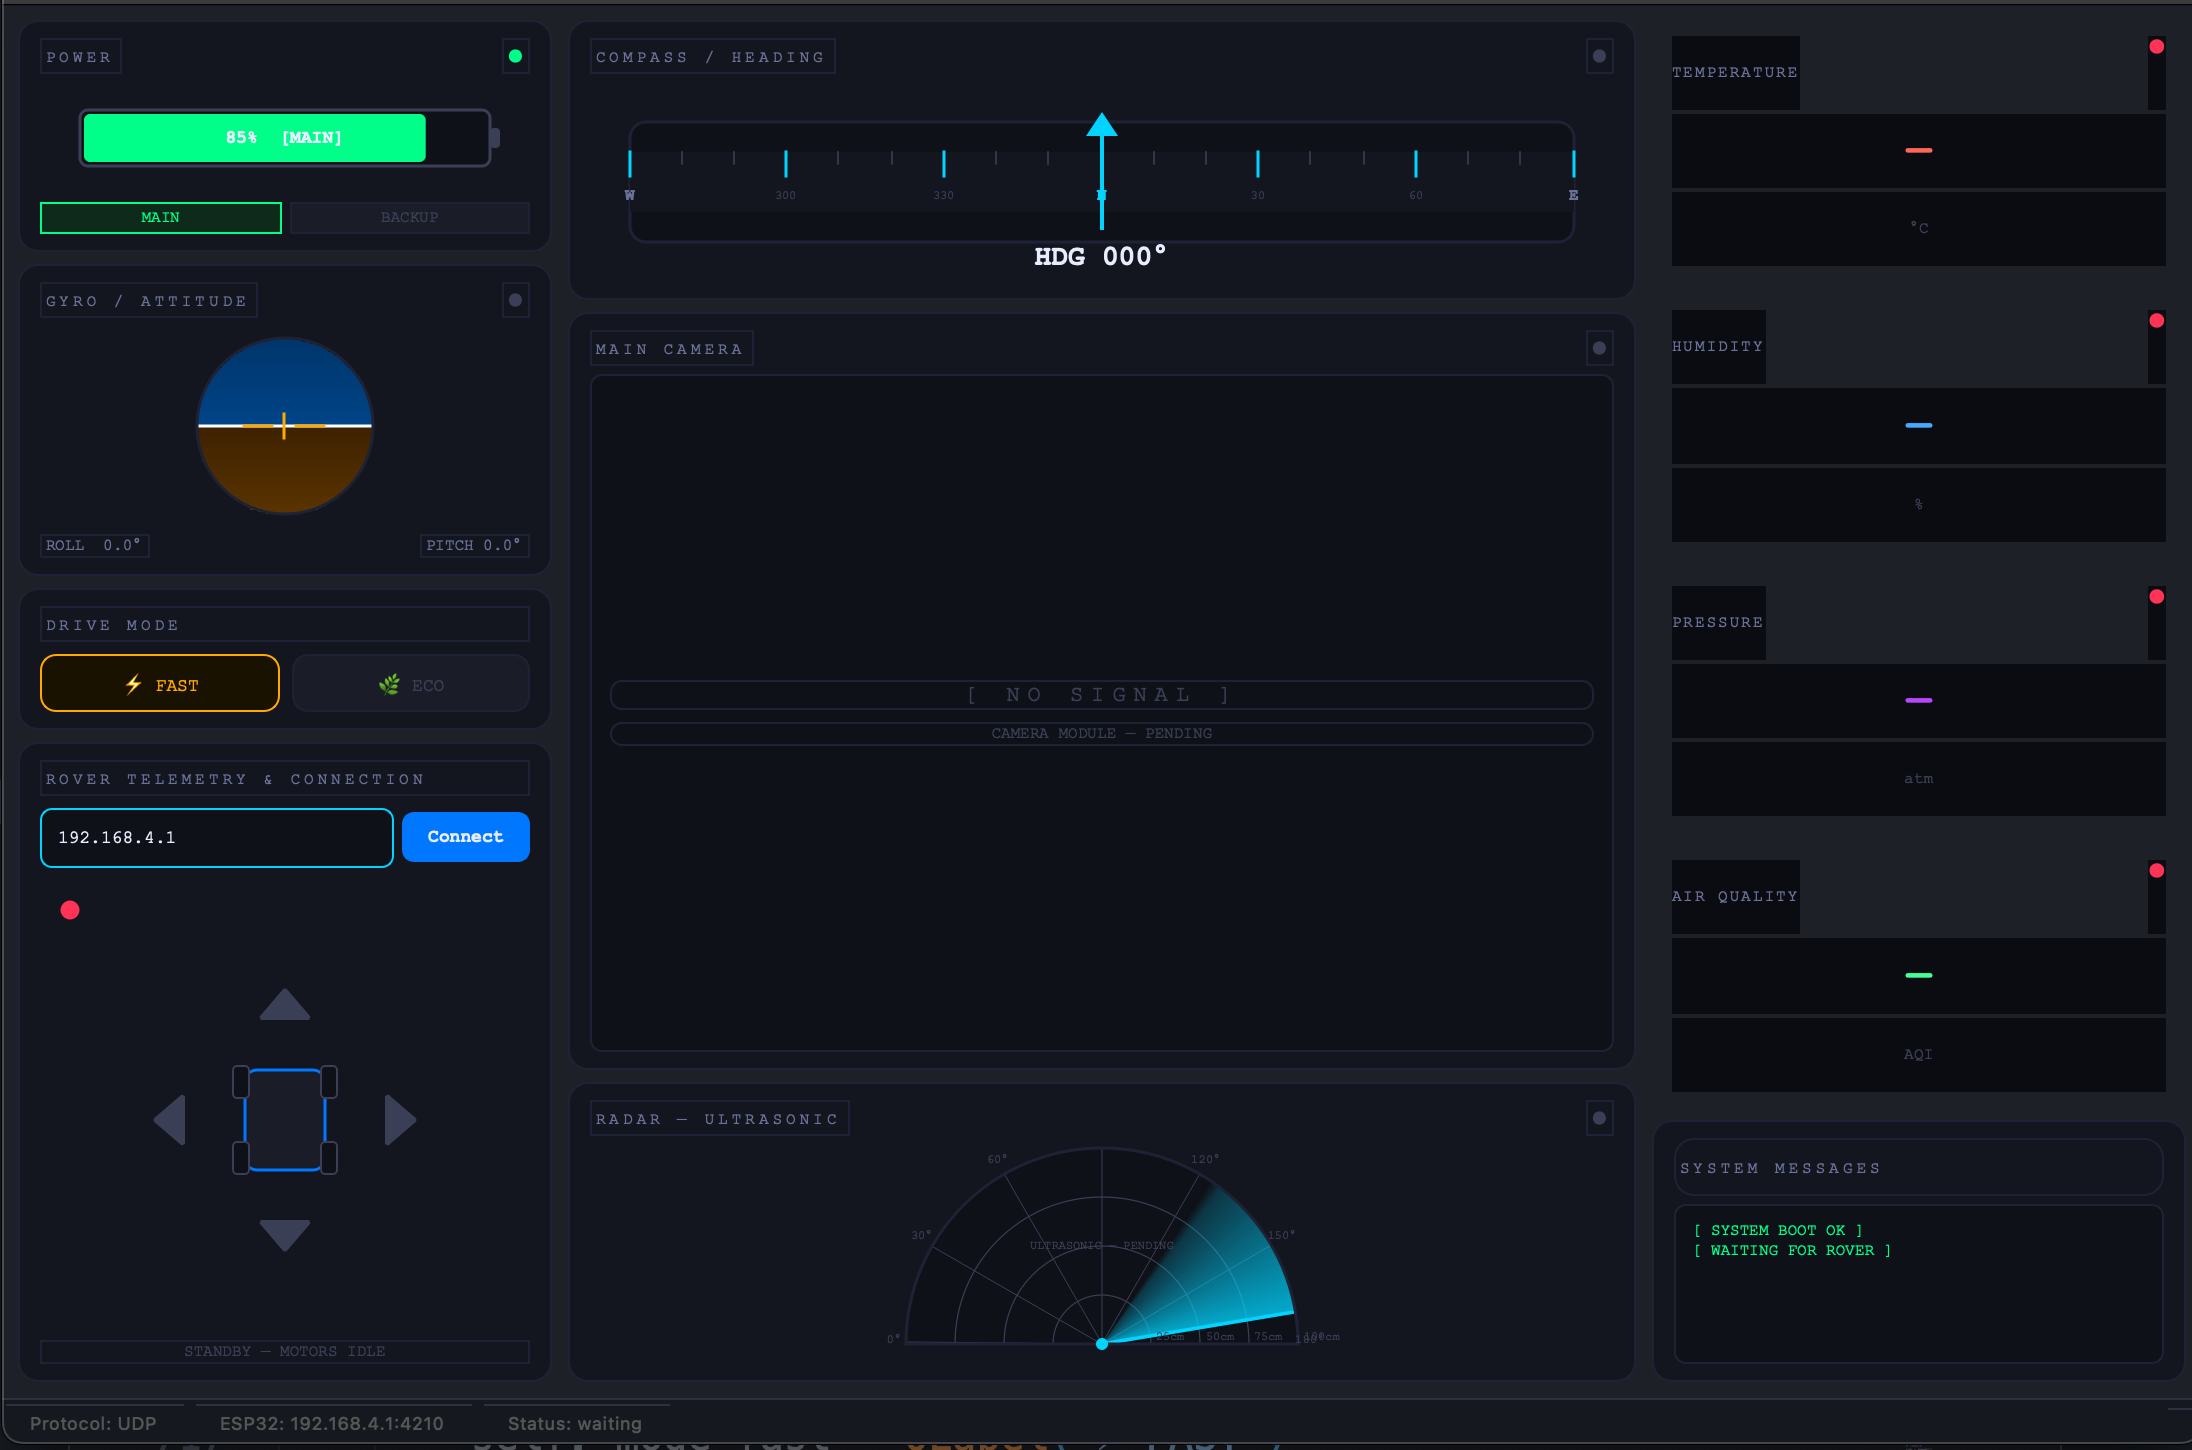
\includegraphics[width=\linewidth]{images/demo/MMS_1st_vers.png}
    \caption{Main user interface of MMS first version }
    \label{fig:mms_ui_demo_1}
\end{figure}

\textbf{Control Signal}
\par
To display the sensor data, the control system defines different ports for sending and receiving messages. For the MMS, there are two signal messages used for control. 
The first is a checking message to confirm that the controller board is connected to the control station. After that, the control signals are transmitted in the form of key-value pairs, 
such as {control: left} and {control: right}.
 

\vspace{0.5em}
\par
Two UDP sockets are created: a transmission socket for sending commands and a reception socket for listening to incoming packets. 
To prevent the graphical user interface (GUI) from freezing during network operations, a dedicated background thread continuously monitors incoming UDP messages. The \verb|start()| method initializes 
the receiver socket and launches the listening thread, while the \verb|stop()| method safely terminates communication and closes all sockets.

\vspace{0.5em}

\par
The \verb|send_command()| function packages motor control instructions, including the movement direction and speed, into JSON format before transmitting them to the ESP32. This structured data format 
simplifies message parsing and enhances communication reliability. The \verb|update_esp_ip()| method allows the target ESP32 IP address to be modified dynamically during runtime, providing flexibility when network configurations change.
The \verb|_recv_loop()| method operates continuously in a separate thread to receive and process incoming UDP packets from the ESP32. Upon receiving data, the JSON.

\subsection{Sensors data transportation protocol: Wifi + UDP}
\par
To connect from MMS to the Rover, we use Wifi \& UDP based protocol,
a lightweight, low latency network protocol designed for low-bandwidth, unreliable networks and 
resource-constrained IoT devices. Maven-01’s main goal is to go to hazardous places and collect environmental information such as pressure, 
temperature, and humidity. Even though the 2.4 GHz Wi-Fi bandwidth is quite large,it is not very stable when the rover is covered by obstacles.
Therefore, we still need UDP for low-latency and robust data transmission.

\par

The WEMOS D1 R32 module creates a local 2.4 GHz Wi-Fi network to establish wireless communication between the rover and the MMS control system. 
Through this connection, control commands and telemetry data are transmitted simultaneously using UDP packets formatted in JSON (for e.g "temperature": 20).
\vspace{1.5 em}

\begin{figure}[H]
    \centering
    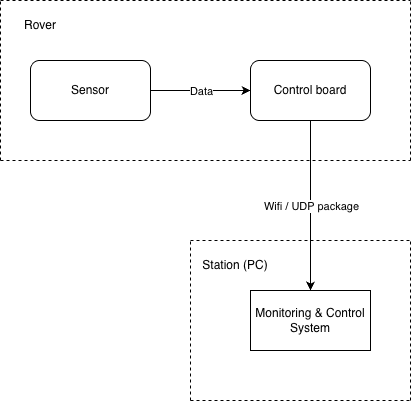
\includegraphics[width=0.7\linewidth]{images/diagram/sensors_data_udp.png}
    \caption{Sensor data transportation workflow diagram}
    \label{fig:udp_sensor_diagram}
\end{figure}


\subsection{Control Protocol: 2.4 GHz Bandwidth Wifi}

\vspace{1em}
\par 
In the previous section, Wifi \& UDP based protocol was discussed as the main protocol used for data transportation, the control communication protocol 
used in the MMS for MAVEN-01 was the same to it. If we look deeper into rover systems and many other UGVs (Unmanned Ground Vehicles), low-latency control
plays a crucial role in overall performance. In MAVEN-01, Wi-Fi serves as the main communication protocol between the rover and the monitoring system, while 
UDP acts as the constant signal transmission protocol.

\vspace{1.5em}
Unlike TCP, which uses a \textit{``make sure the packet is received by the receiver''} mechanism before sending the next packet, UDP removes this confirmation process and continuously sends signals without waiting for acknowledgment. This significantly reduces latency. For this reason, time-critical systems often prefer UDP over other communication protocols.

\vspace{1em}
However, one problem we had to deal with was that the control signals and sensor data might conflict with each other during transmission. To avoid this issue, we set the sending frequency of the control signals higher than the sensor data transmission frequency. This works similarly to two cars not driving parallel to each other on the same road, helping to reduce communication interference and improve the response speed of the rover control system.
\begin{figure}[H]
    \centering
    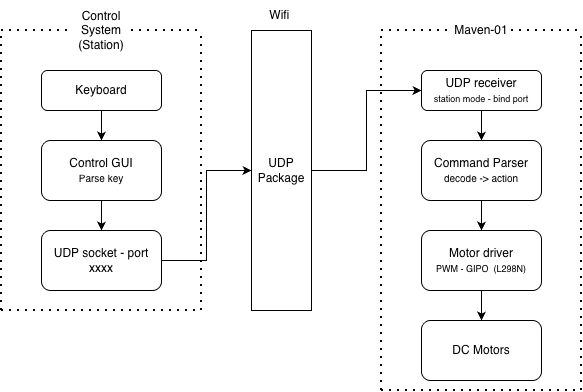
\includegraphics[width=\linewidth]{images/diagram/protocol/control.drawio_new.png}
    \caption{UDP control workflow diagram}
    \label{fig:udp_control_diagram}
\end{figure}


Figure~\ref{fig:udp_control_diagram} illustrates the UDP-based control workflow used in MAVEN-01. The control process begins at the monitoring station, where keyboard inputs are interpreted by the control GUI and transmitted through a UDP socket over a Wi-Fi connection. On the rover side, 
the UDP receiver obtains the transmitted packets and forwards them to the command parser for decoding.The decoded commands are then sent to the motor driver, which controls the DC motors through GPIO signal which is allowed workflow enables low-latency communication for real-time rover control.

\vspace{1em}
During the development and testing phase, MAVEN-01 experienced some issues with connection and signal transport latency. When the WEMOS D1 R32 broadcasts a Wi-Fi signal, by default,
if it does not receive a control signal sent from the control system, it automatically turns off the Wi-Fi module for a very short time to save energy. To solve this problem, we had to turn off the power-saving mode and allow the board to 
broadcast Wi-Fi continuously at all times. However, the trade-off is that the system becomes more power-hungry, so we need a stable and high-capacity power supply for MAVEN-01 to operate properly, which is already mentioned in Section 4.7.